%%%%%%%% ICML 2019 EXAMPLE LATEX SUBMISSION FILE %%%%%%%%%%%%%%%%% 

\documentclass{article} 

% Recommended, but optional, packages for figures and better typesetting: 
\usepackage{microtype} 
\usepackage{graphicx} 
\usepackage{amsmath} 
\usepackage{amssymb} 
\usepackage{cancel} 
\usepackage{subfigure} 
\usepackage{booktabs} % for professional tables 

% hyperref makes hyperlinks in the resulting PDF. 
% If your build breaks (sometimes temporarily if a hyperlink spans a page) 
% please comment out the following usepackage line and replace 
% \usepackage{icml2019} with \usepackage[nohyperref]{icml2019} above. 
\usepackage{hyperref} 

% Attempt to make hyperref and algorithmic work together better: 
\newcommand{\theHalgorithm}{\arabic{algorithm}} 
\newcommand\norm[1]{\left\lVert#1\right\rVert} 

% Use the following line for the initial blind version submitted for review: 
\usepackage{icml2019} 

% If accepted, instead use the following line for the camera-ready submission: 
%\usepackage[accepted]{icml2019} 

% The \icmltitle you define below is probably too long as a header. 
% Therefore, a short form for the running title is supplied here: 
\icmltitlerunning{Learning Continuous Treatment Policy and Bipartite Embeddings for Matching with Heterogeneous Causal Effects} 

\begin{document} 

\twocolumn[ 
\icmltitle{Learning Continuous Treatment Policy and Bipartite Embeddings for Matching with Heterogeneous Causal Effects} 

% It is OKAY to include author information, even for blind
% submissions: the style file will automatically remove it for you
% unless you've provided the [accepted] option to the icml2019
% package.

% List of affiliations: The first argument should be a (short)
% identifier you will use later to specify author affiliations
% Academic affiliations should list Department, University, City, Region, Country
% Industry affiliations should list Company, City, Region, Country

% You can specify symbols, otherwise they are numbered in order.
% Ideally, you should not use this facility. Affiliations will be numbered
% in order of appearance and this is the preferred way.
\icmlsetsymbol{equal}{*}

\begin{icmlauthorlist}
\icmlauthor{Aeiau Zzzz}{equal,to}
\icmlauthor{Bauiu C.~Yyyy}{equal,to,goo}
\icmlauthor{Cieua Vvvvv}{goo}
\icmlauthor{Iaesut Saoeu}{ed}
\icmlauthor{Fiuea Rrrr}{to}
\icmlauthor{Tateu H.~Yasehe}{ed,to,goo}
\icmlauthor{Aaoeu Iasoh}{goo}
\icmlauthor{Buiui Eueu}{ed}
\icmlauthor{Aeuia Zzzz}{ed}
\icmlauthor{Bieea C.~Yyyy}{to,goo}
\icmlauthor{Teoau Xxxx}{ed}
\icmlauthor{Eee Pppp}{ed}
\end{icmlauthorlist}

\icmlaffiliation{to}{Department of Computation, University of Torontoland, Torontoland, Canada}
\icmlaffiliation{goo}{Googol ShallowMind, New London, Michigan, USA}
\icmlaffiliation{ed}{School of Computation, University of Edenborrow, Edenborrow, United Kingdom}

\icmlcorrespondingauthor{Cieua Vvvvv}{c.vvvvv@googol.com}
\icmlcorrespondingauthor{Eee Pppp}{ep@eden.co.uk}

% You may provide any keywords that you
% find helpful for describing your paper; these are used to populate
% the "keywords" metadata in the PDF but will not be shown in the document
\icmlkeywords{Machine Learning, ICML}

\vskip 0.3in
]

% this must go after the closing bracket ] following \twocolumn[ ... 

% This command actually creates the footnote in the first column 
% listing the affiliations and the copyright notice. 
% The command takes one argument, which is text to display at the start of the footnote. 
% The \icmlEqualContribution command is standard text for equal contribution. 
% Remove it (just {}) if you do not need this facility. 

%\printAffiliationsAndNotice{}  % leave blank if no need to mention equal contribution 
\printAffiliationsAndNotice{\icmlEqualContribution} % otherwise use the standard text. 

\begin{abstract} 
Causal Inference algorithms estimate treatment effects to help make action decisions. Most methodologies make decisions on a single dimension of outcome, on a single treatment instance, and with a binary treatment decision variable. For instance, estimate the improvement in one of patient's symptom given the treatment, compared with no treatment at all. These methods fail to capture continuous space action policy with a measure for intensity and complexity of treatment. Most algorithms also lacks consideration for cross-effects when we match treatment subjects with the selection of treatment types. Finally, previous methods do not focus on combined effectiveness of multiple outcomes in a holistic, population wide outcome. 

%a patient or user, and make the assumption of binary treatment variables, which fail to capture a multitude of action complexities. %Most methods regression for direct estimation of outcome counterfactuals, but fail to capture holistic effectiveness, such as the balance of cost versus benefit. 

We take a causal perspective and propose a ubiquitous treatment effect optimization framework with deep learning. This framework works with a continuous policy function that maps to intensity or complexity of treatment. This function can be directly optimized for best results. The algorithm deals with matching instances, for example, user with a product, medication to a patient, thus expands to a multitude of treatment complexities with those matches. Finally, we utilize novel deep learning methods to optimize the desired metric space rather than only predicting single dimensional treatment counter-factual, this approach employs a population-wide effectiveness measure and significantly improves overall holistic efficiency. We demonstrate effectiveness of our models which surpasses prior art. 

We demonstrate the superior performance of our algorithms observe a X\% improvement when using generic continuous space treatments. This captures subtle variations in treatment space, structures the most efficient optimizations, and opens up many application arenas. 
\end{abstract} 

\section{Introduction} 
\label{sec:intro} 

Given a number of patients and a number of medication treatments, how do we decide the medication to match each patient, and the extent of the treatment? The results of the treatment offer guidance to this optimization, to maximize the desired treatment effect. What are the complexities if we take into account the overall effectiveness with healing improvements, side-effects, and patient experience? 

Past work in causal inference and machine learning provided algorithms to solve components of the problem. The main problem is to estimate treatment effect, or improvement observe from the subject, if we offer her treatment compared with no treatment. This is a `counterfactual'~\cite{pearl} or 'what-if' argument. Given enough data, the approach can be used to estimate the multitude of counterfactual outcomes, then decisions can be based on weighted measures. In fact multiple works in the literature including highly effective models such as ~\cite{rlearner}, based on the estimation of the counterfactual provided by the Average Treatment Effect function$\tau$. The above-mentioned approach is highly costly due to the number of models we need to train for all treatment matching options for medications, and also the number of outcomes, such as patient experience, or rare side-effect cases. The approach is also less effective since the matching can be correlated with sub-factors such as multiple medications dealing with infection, or correlation across complexities in matching and outcomes. 

Our solution is based on constructing a learning objective using a bayesian decomposition. We decompose the posteriors in the ATE $~\tau$ function's expected value computation, using bayesian decomposition into three components. The first being the instance effectiveness measure, such as user susceptibility to treatment, the second is the likelihood of matching with a treatment type, and the third term is a continuous space action policy for treatment intensity. With these three components and compose of the effectiveness measure which is posterior in the ATE function's weighting. These three components are then parameterized using deep learning models to enable optimization on three separate segments of our study. Finally, we construct a combined objective function with multiple ATE $tau$ functions to account for the multitude of outcomes, e.g. in the patient's treatment event. 

Our proposal offers the application of continuous space treatment policy. Instead of evaluating the counterfactual of the outcome if a binary treatment, we assume the treatment is given at continuous levels like the dose of medication or price of a product. We apply continuous distributions that measure likelihood of treatment intensity, and re-weight with the prior distribution. The method, based on bayesian decomposition, offers a generic measure of how the intensity of the treatment affects its effectiveness. Using this methodology, we are able to answer questions such as 'what is the optimal level of treatment we can give for a specific subject?' and 'how is effective is the treatment if it were given 53\%?', and apply to problems without constraint to binary treatment decisions. 

To resolve formulation of matching the subject with multiple treatment types, we use a bipartite embedding approach combined with multi-layer neural networks. As with above, Bayesian decomposition also factors the effectiveness measure for matching of two items, and we use a deep learning method for parameterization. With layers of neural networks, the features are projected into embedding space and applied a distance measure for relevance matching. This is analogous to applications in learning-to-rank. 

At the heart of our proposal is the Bayesian decomposition and its combination with deep learning methods. We derive from first principles the causal treatment effect functions, and represent the treatment effect with effectiveness representations, the representations are decomposed into a chain of probabilities that translate to continuous policy likelihood, the matching likelihood and subject instance prior. The Bayesian decomposition is then parameterized with deep learning algorithms and construct eventual objective using multiple treatment effect functions. The objective error is then back-propagated into the parameterization, eventually optimized with quasi-newton methods, and numerical optimizers. The powerful combination of Bayesian decomposition and deep learning offer the methodology to represent continuous treatment policy and bipartite embeddings for matching, enabling the highly effective techniques for causal learning. Overall, we we provide an algorithmic framework to optimize for the overall effectiveness of treatments, including the Bayesian decomposition into a larger set of controllable decision factors. With the critical decision factors, we can perform learning on the eventual sophisticated objective function that can be arbitrarily defined. Novel contributions of this paper are: 

%\begin{itemize} 

%\item \textbf{Heterogeneous Treatment Effect based Business Decisions} - A common approach for user promo decisions relies on regular predictions, redemption or heuristics which are tied to specific scenario and require rich background context. In this paper we propose a general framework that directly optimizes the heterogeneous treatment effect and could be applied to various business use cases with minimum change. This approach can be evaluated effectively and give guidance to decisions. 

\textbf{Deep Learning with Causal Effectiveness Objective} - We derive from first principles the causal inference objective function to optimizes for treatment effectiveness. Instead of estimating treatment effects of a single outcome, we The objective is generalized into a casual learning loss function that can be utilized in deep learning models. We demonstrate superior algorithmic flexibility of this modeling framework evidenced by experimentation. 
%We develop methodologies in deep learning to dynamically focus on important users and incorporate resource constraints, such as limited budget, into the optimization algorithm. 

\textbf{Continuous Treatment Policy } - We are the first to study continuous treatment intensity into the causal machine learning framework. In this framework, we are able to decompose out the treatment decision and formulate as continuous distributions. Using Bayesian decompositions we define arbitrary continuous and learnable distribution that generates the effectiveness measure and optimize for the eventual objective, while leveraging its training signal to determine optimal continuous treatment level. 

\textbf{Bipartite Embeddings for Relevance Matching} - Compared with previous research, our proposal makes decisions on subject instance being matched with types of treatment, rather than only considering subject instance scoring for treatment. We consider the likelihood of match in the perspective of \emph{relevance matching} of bipartite instances, and formulate embedding spaces for both subject instance and matched instance. For example, this can be patient with medication, customer with products. 
%\item \textbf{Optimization for Aggregated Treatment Efficiency} - Most research studies focus on treatment effect of one single outcome. %However, in real-world applications it’s necessary to consider treatment effect on the cost, i.e. the efficiency ratio of  $\delta$cost/$\delta$value when making the resource allocation decision. Common approach also only considers point estimates but our objective is to maximize effectiveness from aggregated treatment effect. Our proposed framework will solve these two challenges together. 

\textbf{Dynamic Pooling and Combined Optimization} - We formulate a dynamic pooling algorithm for creating pooling modules with sort operations in the ordinal matching scenario. These modules form models to create sparse connections in deep networks, induce invariance while allows overall metric to be corrected through parameter changes in lower layers. This is an all-purpose model that can be used to model both population-wide efficiency, and treatment effects when combined with the deep learning effectiveness objective. 
%\end{itemize} 

The structure of this paper is as follows: in Section~\ref{sec:related_work}, we will cover related work in optimization of treatment effect. In Section~\ref{sec:algorithms}, we make the problem statement and introduce effectiveness measures and our modeling approaches for treatment effect optimization. In Section~\ref{sec:empirical_results}, we will cover experimentation, results, comparisons across models and real-world performance from the product we launched. Finally we briefly cover future research steps. 

\section{Prior Work} 
\label{sec:related_work} 
%Methods optimizing for user retention have been widely studied. Two recent studies by Halperin et al. [1] and Cohen et al. [2]  look into the effect of apology treatments when the user's trust is compromised. Andrews et al. [19] studied factors that affect coupon redemption. Hanna et al. [20] and Manzoor and Akoglu [21] investigated factors that influence redemption of time limited incentives. These studies focus on redemption or exploratory average treatment effect and do not explore the optimization of user selection. 

The space of causal inference has been studied in view of treatment effect estimation ~\cite{shalit2017estimating} which uncovers a range of algorithms by balancing representation space, ~\cite{louizos2017causal} discovers hidden confounding factors in combination with algorithms such as variational auto-encoders, ~\cite{parbhoo2018causal} investigates from information bottleneck specific to causal algorithms. In terms of temporal effects, ~\cite{lim2018forecasting} adopted recurrent networks to study the long-term causal effects of sequential treatments. There have been many with application to medical problems and precision medicine~\cite{shalit2017estimating}~\cite{lim2018forecasting}. It's worth noting a classic work~\cite{rubin1974estimating} proposed a paradigm for treatment effect estimation. where the outcome of subject treatment is observed and then used to fit a model for counterfactual estimation. Statistical viewpoints have been taken ~\cite{kunzel2017meta} to decomposes the learning algorithm into composite models with meta-learners. Notably, quasi-oracle estimation by~\cite{nie2017quasi} is effective when estimating the treatment effect in a single outcome. Recently, decision trees and random forests~\cite{chen2016xgboost} have started to be applied~\cite{rzepakowski2012decision}, causal tree and random forests~\cite{wager2017estimation} , boosting~\cite{powers2017some} are applied to build causal inference models. 

Most previous methods consider the \emph{Average Treatment Effect (ATE)} across a single outcome, with shortfalls of not able to deal with continuous treatments, matching with treatment types, and deal with multiple outcomes to trade-off the dimentions. In this work we propose a framework to work with continuous treatment variables, create a paradigm for matching, and aggregate outcome metric space, eventually optimized this framework directly using deep learning. 

\section{Algorithms} 
\subsection{Problem Statement: Matching Algorithm with Continuous Space Policy} 
Consider when a patient, based on her medical history and symptoms, needs to be matched with a treatment. The treatment is characterized with suitable symptoms, and historical statistics. When prescribed, there is a continuous measure for how intense the treatment should be. The goal is match the best treatment, with the optimal treatment intensity. Another example is pricing at an internet company, when a user needs to be matched with any product in the on-line store, and continuous treatment is the price to allocate for the specific user-product match. We solve the matching algorithm with continuous policy with causal learning and optimization with deep learning methods. 

The quasi-oracle estimation algorithm, among other meta-learner algorithms~\cite{kunzel2017meta}, is efficient for estimating conditional treatment effects. However, the Using causal learning derivations, our eventual goal is to maximize an effectiveness measure. For instance, problems in causal learning and reinforcement learning domain trades off the cost of action taking, with the reward obtained by those  actions~\cite{sutton18reinforcement}~\cite{silver16master}~\cite{kool2017cost}. Thus effectiveness is a key theme in applications of causal inference. In this paper, we propose causal inference paradigm to maximize cost effectiveness of heterogeneous treatments. 

%Concretely, we refresh the problem statement. Instead of estimating the treatment effect function $\tau^*(\mathbf{x}) = E(Y_1 - Y_0 | \mathbf{X} = \mathbf{x})$, we propose to solve the problem illustrated below to maximize the gain vs cost ratio. 
%\vspace{-0.3cm}
%\begin{align} 
%\label{eq:pstatement_ratio} 
%\text{minimize} \quad \frac{\bar{\tau}^{*c}(\mathbf{x})}{\bar{\tau}^{*r}(\mathbf{x})} 
%\end{align} 
%The variables $z_i$ represent whether we offer a reward to the user during a campaign and $B$ is the cost constraint. We represent retention treatment effects as $\tau^{*r}(\mathbf{x}^{(i)}) = E(Y_1^r - Y_0^r | \mathbf{X}^{(i)} = \mathbf{x}^{(i)})$ and cost as $\tau^{*c}(\mathbf{x}^{(i)}) = E(Y_1^c - Y_0^c | \mathbf{X}^{(i)} = \mathbf{x}^{(i)})$. It is important to note these treatment effect values are part of the optimization objective and are implicitly modeled as intermediate quantities. They are not strictly regression functions, and we holistically solve the stated problem. 

%\subsection{Defining the Objective from Causal Inference} 
The approach described in the previous section contains two separate steps, treatment effect prediction and constraint optimization. 

The objective for our algorithm is identify a \emph{collection of treatment sessions} to achieve highest effectiveness, each \emph{treatment session} is composed of \emph{a pair of subject and treatment candidate}. This does not rely on individual prediction of treatment effect, but rather, achieves the overall holistic effectiveness. %This is similar to the search ranking algorithm to optimize for a holistic ranking objective vs Click Through Rate (CTR) point  estimate~\cite{huang2013learning}~\cite{shen2014a}. We aim to achieve better performance by combining these two steps together. 

In order to formulate the problem, we introduce a notation of \emph{the overlined treatment effect} $\overline{\tau}^{*}(\mathbf{x}) = E(Y_1 - Y_0 | \mathbf{X} = \{\mathbf{x}^{(i)}\})$, this represents a representation of the treatment effect function across the collection of subjects $\{\mathbf{x}^{(i)}\}$. Also we may refer to parameterization of models using parameters $\mathbf{\theta}$ and effectiveness measures $p_{\mathbf{\theta}}(\mathbf{x}^{(i)})$ per session $i$. The models outputs effectiveness measures to correlate with the expectation across the collection, e.g. $~\overline{\tau}^{*}(\mathbf{x}) = \sum_i p(\mathbf{x}^{(i)})Y_1^{(i)} - \sum_j p(\mathbf{x}^{(j)})Y_0^{(j)}$ thus combined into the same expression using $\overline{\tau}^{*}(\mathbf{x})$. 

Note this critical step to define objective in the casual deep learning paradigm to represent a Treatment Effect Function with a parameterization of multiple deep learning models. We then are able to represent the eventual objective function with a combination of multiple $\overline{\tau}^{*}(\mathbf{x})$. For instance, a model tries to solve unconstrained optimization problems: 
\begin{align} 
\label{eq:pstatement_unconstrained_opt} 
\text{maximize} \quad &\overline{\tau}^{*q}(\mathbf{x})(\overline{\tau}^{*r}(\mathbf{x}) - \overline{\tau}^{*c}(\mathbf{x})) \\ 
\text{minimize} \quad &\frac{\overline{\tau}^{*c}(\mathbf{x})}{\overline{\tau}^{*r}(\mathbf{x})} + \overline{\tau}^{*m}(\mathbf{x}) 
\end{align} 

%and cost $\overline{\tau}^{*c}(\mathbf{x}) = E(Y_1^c - Y_0^c | \mathbf{X} = \{\mathbf{x}^{(i)}\})$ are expectations across selected user portfolio. 

The first problem represents a scheme to maximize a combined treatment effect of gain minus cost weighed by success rate. We aim to optimize for this holistic effectiveness. The cost per unit gain objective allows us to take all users and outcomes into consideration. The unconstrained optimization allows us to utilize deep learning to build flexible models and efficiently train with large-scale data. 

%We derive the objective function stated in Problem~\ref{eq:pstatement_unconstrained_opt}. 

\textbf{Bayesian Decomposition with Causal Inference.} Without loss generality we include per sample treatment propensity from causal statistics~\cite{lunceford04stratification} and derive $\bar{\tau}$ without superscript as it could extend to both $\bar{\tau}^{*r}$ and $\bar{\tau}^{*c}$. Start from the fundamental definition of treatment effect: 
\begin{align*} 
\bar{\tau}^{*} &= E(Y_1 - Y_0) = E(Y_1) - E(Y_0) 
\end{align*} 
The above treatment effect term is influenced by treatment policy thus given a certain policy $\mathbb{P}$, we can write: 
\begin{align*} 
\bar{\tau}^{*} &= E(Y_1 - Y_0 | \mathbb{P}) = E(Y_1 | \mathbb{P}) - E(Y_0 | \mathbb{P}) 
\end{align*} 

Different from prior work~\cite{lunceford04stratification} in Causal Inference, we differentiate the Policy $\mathbb{P}$  with the treatment cohort indicator $T$, the latter $T$ random variable indicates whether an instance is in the treatment cohort or in the control cohort. Only within the treatment cohort, the Policy $\mathbb{P}$ is applied. The Policy can be optimized to produce the best possible outcome in treatment cohort, when treatment cohort variable is correlated with whether assign instances to control or held-out cohort. The propensity in the context of a possible policy evaluation, is the expected value of treatment cohort indicator. 

From~\cite{lunceford04stratification}, the expected value of outcome of any instance can be written as following equations. This takes Treatment Cohort Indicator and propensities into account: 
%\footnote{$E(Y_1) = E(\frac{Y_1}{e(X)} e(X)) = E(\frac{Y_1}{e(X)}E(T | X)) = E(\frac{Y_1}{e(X)}E(T | X, Y_1)) = E(E(\frac{Y_1T}{e(X)} | X, Y_1)) = E(\frac{Y_1T}{e(X)})$}
\begin{align} 
E(Y_1 | \mathbb{P}) = E(\frac{Y_1T}{e(\mathbf{x})} | \mathbb{P}),  \quad E(Y_0 | \mathbb{P}) = E(\frac{Y_0 (1-T)}{1-e(\mathbf{x})}| \mathbb{P})
\end{align} 
$e(\mathbf{x})$ is a propensity function $E(T=1|\mathbf{X} = \mathbf{x})$. This quantity is estimated given features of the instance, thus can be discriminative per instance. For instance, a learnable propensity function fitted with the feature and treatment cohort indicator labels. Detailed proof of the above equation is given for $Y_1$ case: $E(Y_1) = E(\frac{Y_1}{e(\mathbf{x})} e(\mathbf{x})) = E(\frac{Y_1}{e(\mathbf{x})}E(T | \mathbf{X}=\mathbf{x})) = E(\frac{Y_1}{e(\mathbf{x})}E(T | \mathbf{X}=\mathbf{x}, Y_1)) = E(E(\frac{Y_1T}{e(\mathbf{x})} | X, Y_1)) = E(\frac{Y_1T}{e(\mathbf{x})})$\footnote{Third step follows from unconfoundedness assumption~\cite{lunceford04stratification}~\cite{nie2017quasi}.} 

Substitute into the treatment effect definition: 
%As stated above, users are evaluated with an \emph{effectiveness measure}, $p_i$. This measure is across all users, and semantics of a larger $p_i$ is the user is more cost-efficient to send treatment, thus more likely to be selected into our portfolio. 
\vspace{-0.1cm} 
\begin{align} 
\label{eq:drm_propensity_1} 
\begin{split} 
\bar{\tau^{*}} &= E(Y_1 - Y_0 | \mathbb{P}) = E(Y_1 | \mathbb{P}) - E(Y_0 | \mathbb{P}) \\ 
&= E(\frac{Y_1T}{e(\mathbf{x})} | \mathbb{P})  - E(\frac{Y_0 (1-T)}{1-e(\mathbf{x})} | \mathbb{P}) \\ 
&= E(E(\frac{Y_1T}{e(\mathbf{x})}|T, \mathbb{P})) - E(E(\frac{Y_0(1-T)}{1-e(\mathbf{x})}|T, \mathbb{P})) \\ 
\end{split} 
\end{align} 
The last step follows from law of total expectation. We then expand the equation and eliminate zero terms: 
\vspace{-0.1cm}
\begin{align} 
\label{eq:drm_propensity_2} 
\begin{split} 
\bar{\tau}^{*} &= P(T = 1) E(\frac{Y_1T}{e(\mathbf{x})}|T = 1, \mathbb{P}) \\ %&  + \cancel{P(T = 0) E(\frac{Y_1T}{e(\mathbf{x})}| T = 0)} \\
%&\quad - \cancel{P(T = 1) E(\frac{Y_0 (1-T)}{1-e(\mathbf{x})}|T = 1)} 
& - P(T = 0) E(\frac{Y_0 (1-T)}{1-e(\mathbf{x})} | T = 0, \mathbb{P}) 
\end{split} 
\end{align} 
%\vspace{-0.1cm} 
%$\bar{\tau}^{*} = P(T = 1) E(\frac{Y_1T}{e(\mathbf{x})}|T = 1) \\   + \cancel{P(T = 0) E(\frac{Y_1T}{e(\mathbf{x})}| T = 0)} \\
%\quad - \cancel{P(T = 1) E(\frac{Y_0 (1-T)}{1-e(\mathbf{x})}|T = 1)} - P(T = 0) E(\frac{Y_0 (1-T)}{1-e(\mathbf{x})} | T = 0)$  

%For each user, we use $p_i$ as a relaxation of the binary decision variable $z_i$ in the previous problem, the effectiveness weighting to select user $i$. The higher the $p_i$, the higher likelihood of selecting the sample, and we constrain $\sum p_{i, T_i = 0} = 1$, $\sum p_{i, T_i=1} = 1$, i.e. the effectiveness measures for users in the treatment cohort, and control cohort sums to $1$ respectively. This normalization gives the effective measure a probabilistic interpretation. 
We expand expectation in the following equations. Every match is decomposed into two instances of the items being matched, which denote with random variables $I$ and $J$ indexed by $i$ and $j$. We define $\hat{e}$ to be the overall propensity, or likelihood of being in the treatment cohort across all instances. For each user, the $e(\mathbf{x})$ term is estimated from a pretrained propensity function. In the last equation, we introduce Matches of instances denoted by random variable $M$, and use the tuple notation $M=(I, J)$ and $m = (i, j)$ to indicate each match across two distinct items. 
\small
\begin{align} 
\label{eq:bayes_weighted_tau} 
\bar{\tau}^{*} &= \hat{e} \sum_{T_{i,j} = 1}\frac{p( I=i, J=j | \mathbb{P}^{(i,j)})}{e(\mathbf{x})} Y_1^{(i,j)} \\ & - (1 - \hat{e}) \sum_{T_{i, j} = 0} \frac{p( I=i, J=j | \mathbb{P}^{(i, j)})}{1-e(\mathbf{x})} Y_0 ^ {(i,j)} \\ 
%&= \hat{e} \sum_{T_m = 1} p( M = m | \mathbb{P}^{(m)}) Y_1^{(m)} \\ & - (1 - \hat{e}) \sum_{T_m = 0} p( M = m | \mathbb{P}^{(m)}) Y_0 ^ {(m)} \\ 
& = \hat{e} \sum_{T_{m} = 1} \frac{p(M=m) p(\mathbb{P}^{(m)} | M=m )}{e(\mathbf{x})\sum_l p(M=l)p(\mathbb{P}^{(l)} | M=l)} Y_1^{(m)} \\
&  - (1 - \hat{e}) \sum_{T_m = 0} \frac{p(M=m ) p(\mathbb{P}^{(m)} | M = m) }{(1-e(\mathbf{x}))\sum_l p(M=l)p(\mathbb{P}^{(l)} | M = l)}Y_0 ^ {(m)} 
\end{align} 
\normalsize 
The last two lines are obtained using Bayes Rule to replace the posterior $p( I=i, J=j | \mathbb{P}^{(i,j)})$ with $\frac{p(M=m) p(\mathbb{P}^{(m)} | M=m )}{Z} $, prior multiplied by likelihood, divided by the normalization factor or partition function $Z$. 

As stated before, we parameterize the above function, then combine the Treatment Effect Functions $\overline{\tau}^{*}$, we will be able to compose an objective function for the learning algorithm. 

\textbf{Parameterize continuous policy model.} We next parameterize the action policy model. The key to defining an objective function composed of conditional average treatment effect (CATE) representations with $\tau^*$ is finding representations for the likelihood $p(\mathbb{P} | M = m)$, the probability of a policy given a match, and prior $p(M = m)$, the probability of a match in the previous equation. In this paper, we first solve the problem with a continuous policy problem statement. This is to say, we assume the random variable $\mathbb{P}$ to be a continuous random variable. For instance, we limit its range $\mathbb{P}\in [0, 1]$ as intensity of treatment. Given any specific match, we formulate regression models 
\begin{align} 
\label{eq:bell_mean} 
s(\mathbf{x}_i, \mathbf{y}_j)_{\mathbb{P}} = f(\mathbf{x}_i, \mathbf{y}_j) 
\end{align} 

Here the feature vectors $\mathbf{x_i}$ and $\mathbf{y_j}$ denote features to specify the match subject $i$ and object $j$, e.g. user and product, patient and treatment. There is a prediction model for the best treatment intensity $s_{\mathbb{P}}$ for this specific match of subject and object. Note we can construct any number of these regression models. We can implement this regression function with any differentiable function, such as a logistic regression, or multi-layer neural network. We can define the likelihood $p(\mathbb{P} | M = m)$ to be the following: 

\begin{align} 
p(\mathbb{P} | M = m) \propto \sigma (1 - \sigma) (s(\mathbf{x}_i, \mathbf{y}_j)_{\mathbb{P}}) 
\end{align} 

Where $\sigma$ denotes the sigmoid function $\sigma(x)=\frac{1}{1 + \exp^{(-x)}}$ and $\sigma (1 - \sigma)$ is the derivative of the sigmoid function. This formulation gives the likelihood a probabilistic interpretation, such that the cumulative density of the random variable takes forms of the sigmoid, and the probabilistic density takes a bell-shaped form. This means whenever the intensity $\mathbb{P}$ deviates from the optimal, the likelihood function penalizes by lowering the value, positioning the highest value at top of bell curve at the regressed value in equation~\ref{eq:bell_mean}. 

Alternatively, we can define the likelihood as:  

\begin{align} 
p(\mathbb{P} | M = m) = Beta(\mathbb{P}, \alpha(\mathbf{x}_i, \mathbf{y}_j), \beta(\mathbf{x}_i, \mathbf{y}_j)) 
\end{align} 

Where the random variable $\mathbb{P}$ assumes a density of a Beta distribution with parameters $\alpha, \beta$ which are derived with a regression function from feature sets $\mathbf{x}$ and $\mathbf{y}$. This second formulation has the interpretation for variable $\mathbb{P}$ to be exactly in range of $[0, 1]$, and if both parameters are limited to be above $1.0$, the distribution also takes the hump shape with optimal at $\frac{\alpha}{\alpha + \beta}$. 
%Then, we expand the expectation terms $E(\frac{Y_1T}{e(\mathbf{x})}|T = 1)$, $E(\frac{Y_0 (1-T)}{1-e(\mathbf{x})} | T = 0)$ using the normalized effectiveness weighting, potential outcomes $Y^{(i)}_1$, $Y^{(i)}_0$ and observed outcome labels $Y^{(i)}$: 

\textbf{Parameterize subject-candidate matching model.} We next parameterize the matching model model. 
We can decompose the following equation: 
\begin{align} 
\label{eq:matching_func} 
p(M = m) =& p (I = i, J = j) \\ =& p(I = i) p(J = j | I = i) \\ \propto& g(\mathbf{x}_i) m(\mathbf{x}_i, \mathbf{y}_j) 
\end{align} 

A simple form of $g$ is a sigmoid compressed version of arbitrary differentiable regression function, and forms the base instance weighting model. With sigmoid as the non-linearity, the outputs are positive and are well-controlled below $1.0$. 

For the functional form of $m$ we adopt a bipartite embedding formulation. First the input features $\mathbf{x}$ are projected with a neural network to an embedding space for both subject instance, and matching candidate: $\mathbf{e}_i = f_{sp} (\mathbf{x}_i), \mathbf{e}_j = f_{cp} ( \mathbf{y}_j )$. In this manner, the embedding space can be learned using eventual effectiveness measures, across the treatment subjects, e.g. patient, as well as the treatment candidates, e.g. medications. The eventual objective helps to learn the embedding sub-space each of the subject and candidate lies in. Also the algorithm for matching here is highly related to learning-to-rank models such as DSSM~\cite{huang2013learning}. Where the candidates are projected first into a vector space before the metric distance is used to define the relevance of terms. Note that we use the same projection function in the definition of $g$. Then, we can formulate the likelihood function: 

\begin{align} 
\label{eq:matching_func} 
m(\mathbf{x}_i, \mathbf{y}_j) = cos(\phi) + 1 = \frac{\mathbf{e}_i \cdot \mathbf{e}_j}{\norm{\mathbf{e}_i \cdot \mathbf{e}_j}} + 1
%p(M = m) =& p (I = i, J = j) \\ =& p(I = i) p(J = j | I = i) \\ \propto& g(\mathbf{x}_i) m(\mathbf{x}_i, \mathbf{y}_j) 
\end{align} 

With the previously defined likelihood functions, we can sum together to form the partition function in order to normalize the product of prior and likelihood over all possible matches in, each indexed by $l$, written as $\sum_l p(M=l)p(\mathbb{P}^{(l)} | M = l)$. When the partition function can be computed, the posterior can be computed and Equation~\ref{eq:bayes_weighted_tau} can be computed to define the overall objective function. 

\vspace{-0.2cm} 
\begin{align} 
\label{eq:drm_propensity_3} 
\begin{split} 
\bar{\tau}^{*} &= \hat{e} \sum_{T_i =1} \frac{Y^{(i)}_1 p_{i}}{e(\mathbf{x}^{(i)})} - (1-\hat{e}) \sum_{T_i = 0} \frac{Y^{(i)}_0 p_i}{1-e(\mathbf{x}^{(i)})} \\ 
& = \hat{e} \sum_{i=1}^n \frac{1}{e(\mathbf{x}^{(i)})} Y^{(i)}_1 p_{i} \mathbb{I}_{T_i=1} - (1-\hat{e}) \sum_{i = 0}^n \frac{1}{1-e(\mathbf{x}^{(i)})} Y^{(i)}_0 p_i \mathbb{I}_{T_i=0} \\ 
& = \hat{e} \sum_{i=1}^n \frac{1}{e(\mathbf{x}^{(i)})} Y^{(i)} p_{i} \mathbb{I}_{T_i=1} - (1-\hat{e}) \sum_{i = 0}^n \frac{1}{1-e(\mathbf{x}^{(i)})} Y^{(i)} p_i \mathbb{I}_{T_i=0}
\end{split} 
\end{align} 

Eq.~\ref{eq:drm_propensity_3} is a generalized form of the $\bar{\tau}^{*}$ including part of the objective function with propensity weighting. When $\hat{e} = e(\mathbf{x}^{(i)})$ is constant in a fully randomized experiment, the term becomes: %, and the last line uses a sampling approximation, where $p_u(X)$ is the discrete probability density given by user sampler, normalized with respect to treatment and control cohorts, respectively. This sampler could be used as a ranker at inference time to determine the users to apply treatment. 

\vspace{-0.1cm} 
\begin{align} 
\label{eq:drm_propensity_4} 
\begin{split} 
  \bar\tau^{*}=\sum_{i=1}^n Y^{(i)}p_i(\mathbb{I}_{T_i=1} - \mathbb{I}_{T_i=0}) 
\end{split} 
\end{align} 
\vspace{-0.1cm} 

%\textbf{Model and Effectiveness Objective.} Using the above derivations, we can then construct our model and the loss function as follow. In Eq. (\ref{eq:drm_1}) $f$ is the function the model will learn with tunable parameters. This function outputs an effectiveness score, indicating how efficient the sample is based on its features $\mathbf{x^{(i)}}$. $f$ can be in any differentiable form such as linear or a neural network structure. 
%\begin{equation} 
%  \label{eq:drm_1} 
%  S_i = f(\mathbf{x}^{(i)}) 
%\end{equation} 
%We use a standard hyperbolic tangent as non-linear activation for the neural network($\tanh$). 
%\begin{equation} 
%  \label{eq:drm_2} 
%  s_i = \tanh(S_i) 
%\end{equation} 
%We then normalize the effectiveness scores using the softmax function to arrive at $p_i$ for each user (Eq.  (\ref{eq:drm_3_1})). $p_i$ sum to 1 in each cohort respectively, for $T_i=1$ and $T_i=0$. 
%\begin{equation} 
%  \label{eq:drm_3_1} 
%  p_i = \frac{e^{s_i}}{\sum_{j=1}^n\mathbb{I}_{T_j=T_i}e^{s_j}} 
%\end{equation} 
%Here $\mathbb{I}_{T_j=T_i}$ is the indicator function for sample $j$ whether it's in the same group (treatment or control) as sample $i$. 
%It could be expanded as Eq. (\ref{eq:drm_3_2}) and Eq. (\ref{eq:drm_3_3}).
%\begin{equation}
%  \label{eq:drm_3_2}
%  p_{i, T_i=1} = \frac{e^{s_i}}{\sum_{\{j:T_j=1\}}e^{s_j}}
%\end{equation}
%\begin{equation}
%  \label{eq:drm_3_3}
%  p_{i, T_i=0} = \frac{e^{s_i}}{\sum_{\{j:T_j=0\}}e^{s_j}}
%\end{equation} 
%Based on this, we can calculate the expected treatment effect of our user portfolio using the derived Eq.~\ref{eq:drm_propensity_4}. We can write effectiveness weighted sample treatment effect for retention and cost with (Eq. (\ref{eq:drm_4_1}), Eq. (\ref{eq:drm_4_2})).
%\vspace{-0.1cm}
%\begin{equation}
%  \label{eq:drm_4_1}
%  \bar\tau^{*r}=\sum_{i=1}^nY^{r(i)}p_i(\mathbb{I}_{T_i=1} - \mathbb{I}_{T_i=0})
%\end{equation}
%\vspace{-0.1cm}
%\begin{equation}
%  \label{eq:drm_4_2}
%  \bar\tau^{*c}=\sum_{i=1}^nY^{c(i)}p_i(\mathbb{I}_{T_i=1} - \mathbb{I}_{T_i=0})
%\end{equation}
%\vspace{-0.1cm}
%Finally, we have our loss function in Eq. (\ref{eq:drm_5}), which is the ratio of treatment effects as the holistic efficiency measure plus a regularization term.
%\vspace{-0.1cm}
%\begin{equation}
%  \label{eq:drm_5}
%  \hat{f}(\cdot ) = argmin_{f}\left \{ \frac{\bar{\tau^c}}{\bar{\tau^r}}+\Lambda_n(f(\cdot ))  \right \}
%\end{equation}
%\vspace{-0.1cm}
%Since all the operations above are differentiable, we can use any off-the-shelf optimization method to minimize the loss function and learn the function $f$. Because the direct optimization is well suited for deep learning, we incorporated this method with the deep learning architectures and frameworks, and implemented our approach using TensorFlow \cite{abadi2016tensorflow} and used Adam optimizer \cite{kingma2014adam}. The definition of $f$ function is flexible for instance, multi-layer neural networks, convolutional and recurrent networks. 

%\subsection{Dynamic Pooling and Constrained Optimization} 

\section{Experiments} 

\textbf{Benchmark Models} 
\emph{\textbf{Quasi-oracle estimation (R-Learner)}}. We use Linear Regression\footnote{Using SKLearn library's Ridge Regression with 0.0 as the regularization weight.} as the base estimator. Since the experiment cohorts are randomly selected, we use constant treatment percentage as propensity in the algorithm. Since we need to define one CATE function for R-learner, we use the R-learner to model the gain value incrementality with $\tau_r$. 

\emph{\textbf{Causal Forest}}. We leverage the generalized random forest (\emph{grf}) library in R~\cite{wager2018estimation}~\cite{grflink}. For details, we apply causal forest with 100 trees, 0.2 as alpha, 3 as the minimum node size, and 0.5 as the sample fraction. We apply the ratio of two average treatment effect functions in ranking by training two causal forests. To rank users or other cardinalities with respect to cost vs gain effectiveness, we estimate the conditional treatment effect function both for gain ($\tau_r$) and cost ($\tau_c$), i.e. train two Causal Forest models. For evaluation, we compute the ranking score according to the ratio of the two $\frac{\tau_r}{\tau_c}$. 
For hyper-parameters, we perform search on deciles for parameters \emph{num\_trees}, \emph{min.node.size}, and at 0.05 intervals for \emph{alpha}, \emph{sample.fraction} parameters. We also leverage the \emph{tune.parameters} option for the \emph{grf} package, eventually, we found best parameters through best performance on validation set\footnote{Best parameters are the same for all three datasets we experimented: \emph{num\_trees}$=100$ (50 trees for each of the two CATE function, $\tau_r$, $\tau_c$), \emph{alpha}$=0.2$, \emph{min.node.size}$=3$, \emph{sample.fraction}$=0.5$}. 

\emph{\textbf{Simpliflied Session Scoring Model (SSSM)}}. We implement our deep learning based models with Tensorflow. To align with baseline and other methods in our experiments, we use a one layer with linear parameterization $\tanh(\mathbf{w}^T \mathbf{x} + b)$ as the scoring function, without weight regularization, the objective functions stated in the algorithm section are used. We use the Adam optimizer with learning rate 0.01 and default beta values. We compute gradients for entire batch of data, and run for 600 iterations. 

\emph{\textbf{Continuous Policy Bipartite Matching Model (CPBMM)}}. We implement our deep learning based models with Tensorflow. To align with baseline and other methods in our experiments, we use a one layer with linear parameterization $\tanh(\mathbf{w}^T \mathbf{x} + b)$ as the scoring function, without weight regularization, the objective functions stated in the algorithm section are used. We use the Adam optimizer with learning rate 0.01 and default beta values. We compute gradients for entire batch of data, and run for 600 iterations. 

\textbf{Datasets} In the next subsection we offer a detailed description of datasets we used to benchmark the models. 
\emph{\textbf{US Census 1990}} The US Census (1990) Dataset (Asuncion \& Newman, 2007~\cite{uscensulink} contains data for people in the census. Each sample contains a number of personal features (native language, education...). The features are pre-screened for confounding variables, we left out dimensions such as other types of income, marital status, age and ancestry. This reduces features to d = 46 dimensions. Before constructing experiment data, we first filter with several constraints. We select people with one or more children (\emph{`iFertil'} $\leq$ 2), born in the U.S. (\emph{`iCitizen'} = 0) and less than 50 years old (\emph{`dAge'} $<$ 5), resulting in a dataset with $225,814$ samples. We select `treatment' label as whether the person works more hours than the median of everyone else, and select the income (\emph{`dIncome1'}) as the gain dimension of outcome for $\tau_r$, then the number of children (`iFertil') multiplied by $-1.0$ as the cost dimension for estimating $\tau_c$. The hypothetical meaning of this experiment is to measure the cost effectiveness, and evaluate who in the dataset is effective to work more hours. 

\emph{\textbf{Covertype Data}} The Covertype Dataset (Asuncion \& Newman, 2007) contains the cover type of northern Colorado forest areas with tree classes,  distance to hydrology, distance to wild fire ignition points, elevation, slope, aspect, and soil type. We pre-filter and only consider two types of forests: \emph{`Spruce-Fir'} and \emph{`Lodgepole Pine '}, and use data for all forests above the median elevation. This results in a total of $247,424$ samples. After processing and screening for confounding variables, we use 51 features for model input. With the filtered data, we build experiment data by assuming we are able to re-direct and create water source in certain forests to fight wild fires, but also like to ensure the covertype trees are not imbalanced by changing the hydrology with preference to `Spruce-Fir'. Thus, the treatment label is selected as whether the forest is close to hydrology, concretely, distance to hydrology is below median of the filtered data. The gain outcome is a binary variable for whether distance to wild fire points is smaller than median, and cost outcome is the indicator for `Lodgepole Pine' (1.0, undesired) as opposed to `Spruce-Fir' (0.0, desired). 

\emph{\textbf{Ponfare Data}} The Ponfare Dataset is a public dataset with a coupons website~\cite{ponfare}, the dataset contains session as row items where the instance contains customer, coupon browsed, a continuous discount percentage, whether or not purchase, and auxiliary information on customer and coupon such as geographical location. We pre-filter the sessions where customers are below the age of 45. Due to disproportion of positive and negative samples, we subsample 4.0\% of sample of sessions that do not result in purchase. The eventual dataset is around 130,822 samples, we utilize discount level as the continuous treatment policy, and use the median of the level to segment out sessions into treatment and control groups, respectively. 

Figure~\ref{fig:uscensus_result} shows results of causal models on US Census. The baseline R-learner on gain performs slightly better due to less cost impact. Duality R-learner still works reasonably well. Direct Ranking and Constrained Ranking out-performs Duality R-learner by \emph{2.8\%} and \emph{21.2\%}, respectively to AUCC \emph{0.58} and \emph{0.69}. 
\begin{figure}[h] 
  %\centering 
  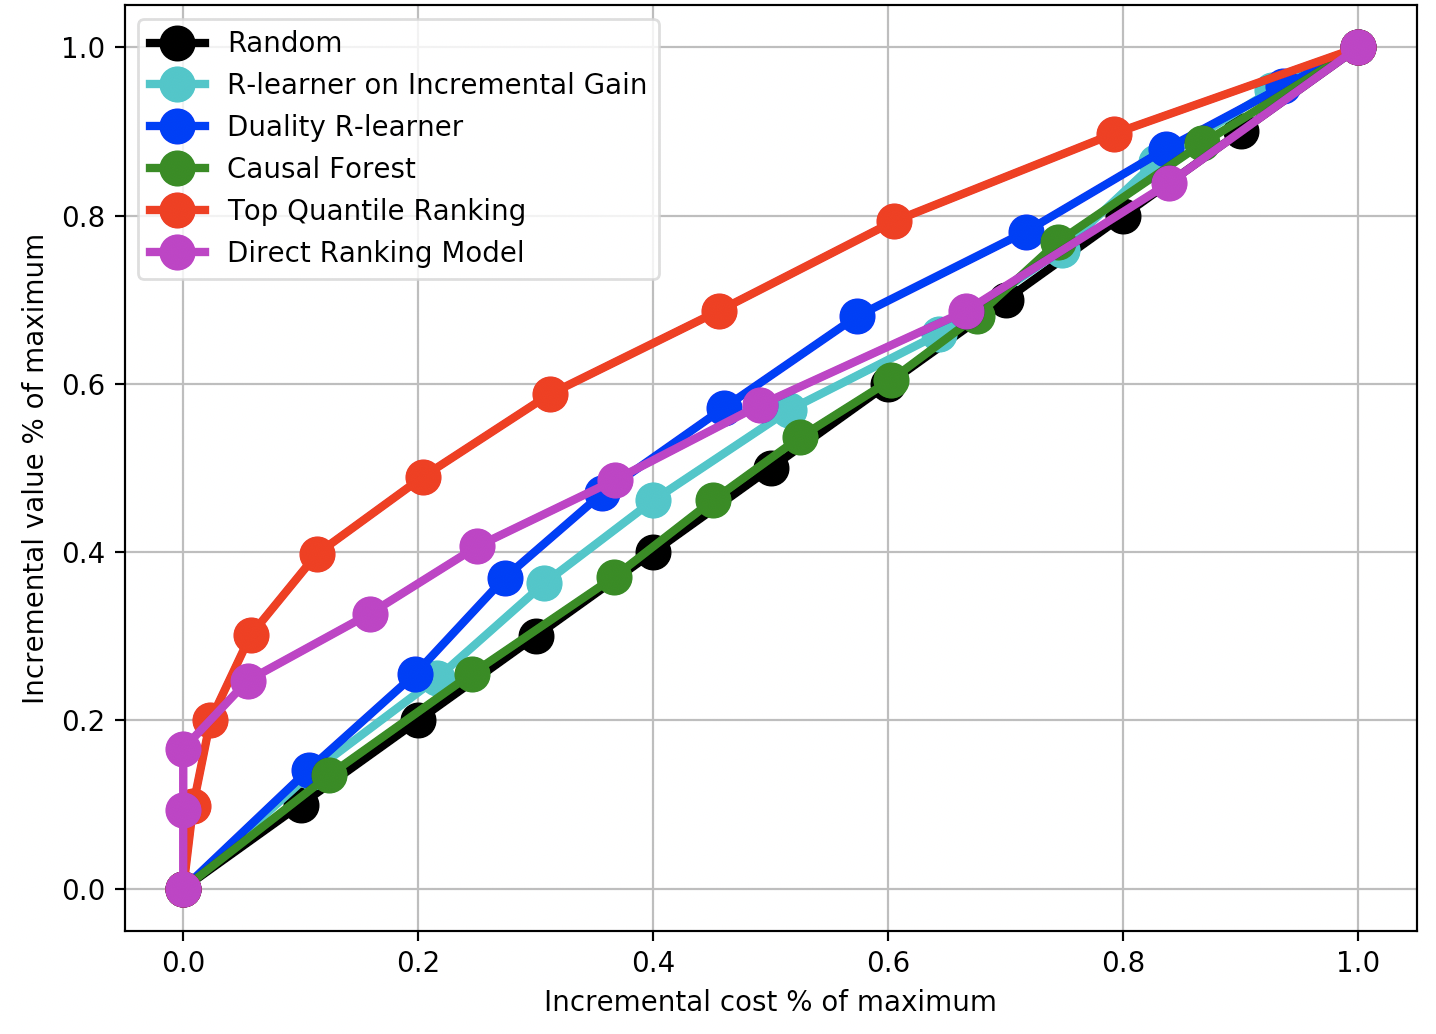
\includegraphics[width=0.75\linewidth]{figures/uscensus_result} 
  \caption{Cost-Curve results for public US Census data.} 
  \label{fig:uscensus_result} 
\end{figure} 
\vspace{-0.1cm} 
Figure~\ref{fig:covtype_result} shows results of causal models on Covtype datasets. The optimization problem on this dataset is easier as results on multiple models are better. Direct Ranking and Constrained Ranking out-performs Duality R-learner by \emph{7.3\%} and \emph{17.9\%}, with AUCC for Constrained Ranking algorithm as high as \emph{0.92}. 

~\ref{tab:summary_result_table} shows results  algorithms are significantly better, more than \emph{25\%} in terms of AUCC, than R-learner on gain outcome, and out-performs Duality R-Learner by around \emph{10\%}. One example for cost effectiveness is to look at the vertical dash line at $20\%$ of total incremental cost, we can achieve 2X more incremental retention than random selection by using our causal models. This can result in 50\% reduction in cost. 
\begin{table}
  \caption{Summary of AUCC results across models and datasets.} 
  \label{tab:summary_result_table}
  \begin{tabular}{llllll}
    \toprule
    Algorithm & USCensus &Covtype \\ 
    \midrule 
    Random & 0.500 & 0.500 \\
    \midrule 
    R-learner G & 0.533 & 0.779 \\
    Duality R-learner & 0.567 & 0.783 \\
    Causal Forest & 0.510 & 0.832 \\
    Direct Ranking & \textbf{0.583} & \textbf{0.840} \\
    Constrained Ranking & \textbf{0.687} & \textbf{0.915} \\
    \bottomrule
\end{tabular}
\end{table} 

% Acknowledgements should only appear in the accepted version.
%\section*{Acknowledgements}

%\textbf{Do not} include acknowledgements in the initial version of
%the paper submitted for blind review.

%If a paper is accepted, the final camera-ready version can (and
%probably should) include acknowledgements. In this case, please
%place such acknowledgements in an unnumbered section at the
%end of the paper. Typically, this will include thanks to reviewers
%who gave useful comments, to colleagues who contributed to the ideas,
%and to funding agencies and corporate sponsors that provided financial
%support.


% In the unusual situation where you want a paper to appear in the
% references without citing it in the main text, use \nocite
%\nocite{langley00}

\bibliography{references}
\bibliographystyle{icml2019}

\end{document}


% This document was modified from the file originally made available by
% Pat Langley and Andrea Danyluk for ICML-2K. This version was created
% by Iain Murray in 2018, and modified by Alexandre Bouchard in
% 2019. Previous contributors include Dan Roy, Lise Getoor and Tobias
% Scheffer, which was slightly modified from the 2010 version by
% Thorsten Joachims & Johannes Fuernkranz, slightly modified from the
% 2009 version by Kiri Wagstaff and Sam Roweis's 2008 version, which is
% slightly modified from Prasad Tadepalli's 2007 version which is a
% lightly changed version of the previous year's version by Andrew
% Moore, which was in turn edited from those of Kristian Kersting and
% Codrina Lauth. Alex Smola contributed to the algorithmic style files.
